\section{Состав и общая архитектура ПАК}

Разрабатываемый виртуальный полигон предназначен для выполнения имитационного моделирования 
динамики морских объектов под воздействием внешних возмущений. Как следствие, под задачей 
унификации в данном разделе понимается установление взаимосвязей общей (имитационной численной) 
модели динамики судна с «эталонными» моделями, повсеместно используемыми для расчета качки судна 
в оперативных условиях эксплуатации.

В отличие от традиционных моделей динамики судна (например, в форме уравнений движения), 
имитационная модель динамики судна представляет собой не только формализацию основных 
соотношений между входными и выходными данными, но и набор механизмов для проведения 
виртуальных экспериментов, которые должны:

\begin{enumerate}
\item	Обеспечивать настройку параметров имитационного моделирования в широких пределах.
\item	Создавать сценарии моделирования: параметры изменяются не только в начале, но и в процессе моделирования.
\item	Осуществлять интерактивную визуализацию процесса имитационного моделирования для осуществления качественного анализа явлений и отладки.
\item	Обеспечивать экспорт данных, в частности, в пакеты математического моделирования и проектирования.
\end{enumerate}

Таким образом, формой реализации имитационной модели является среда имитационного моделирования, которая содержит следующие специализированные и общие подсистемы:

\begin{enumerate}
	%--------------------------------
	% CORE
	%--------------------------------
	\item	Ядро (\frqt{Core}). В ядро подсистемы входят:
	\begin{enumerate}
		\item	Библиотека математики, которая включается как стандартные математические объекты, 
				такие как вектора, матрицы и кватернионы, так и более сложные, которые включают 
				такие объекты как видовые пирамиды (frustum), ограничивающие объемы (bounding sphere и bounding box).
		\item	Интерпретатор Lua, которые используется для конфигурирования 
				и управления виртуальным полигоном, 
				а также для поддержки подсистемы сценариев.
		\item 	Интерфейс операционной и файловой системы.
		\item	Система конфигурирования.
	\end{enumerate}
	%--------------------------------
	% GF
	%--------------------------------
	\item 	Библиотеки поддержки визуализации (\frqt{Graphic Factory}, собственная разработка), 
			которая независимо от используемого графического API обеспечивает:
			\begin{itemize}
			\item	Загрузку, обработку и сохранение трехмерных полигональных сеток в 
					формате собственной разработки ESX (Extensible Scene XML file). 
					В задачи обработки трехмерных полигональных сеток входят:
					\begin{itemize}
					\item	Разрезание, склеивание, оптимизация геометрии
					\item	Скелетная анимация
					\end{itemize}
			\item	Загрузку, обработку и сохранение двумерных изображений 
					в формате BMP, JPEG, TGA, PNG и другие. 
					Основан на использовании библиотеки FreeImage \citep{freeimage}.
			\item	Загрузку, обработку и сохранение файлов анимации в собственной формате 
					EAX (Extensible Animation XML-file). Файлы анимации могут быть использованы 
					для анимации визуализируемой сцены, анимацию камеры в демонстрационном режиме и др.
			\end{itemize}
	%--------------------------------
	% RS
	%--------------------------------
	\item	Графическая подсистема (\frqt{Reality Sequencer}, собственная разработка) 
			отвечает за подготовку сцены к отображению, построение теней, 
			расчета освещения, пост-обработки, а также отображение элементов пользовательского 
			интерфейса как в моно- так и стерео-режиме. В список графических объектов входят:
			\begin{enumerate}
			\item	Твердые объекты (Solids).
			\item	Водная поверхность (Water)\footnote{Так как генерация взволнованной поверхности 
					осуществляется с использованием графического ускорителя, генератор и визуализатор 
					водной поверхности для упрощения системы объединены в одну подсистему. 
					Обращаясь к графической подсистеме любая другая подсистема может задать 
					спектр волнения и запросить характеристики водной среды в любой точке и любой момент времени.}
			%\item	Объемные скалярные поля (Volume Scalar fields)
			\item	Отладочные линии (Debug lines).
			\item	Элементы пользовательского интерфейса и текст.
			\item	Источники света.
			\end{enumerate}
	%--------------------------------
	% SS
	%--------------------------------
	\item	Звуковая подсистема реализована с использованием \citep{fmod} предназначена для:
			\begin{itemize}
				\item	Воспроизведение Фонового стерео- и квадрофонического звука в 
						форматах Wave PCM, Vorbis OGG, MP3 и др.
				\item	Микширование с наложением эффектов окружения звуков, 
						позиционированных в пространстве, с учетом скорости 
						перемещения и позиции как звуков, так и слушателя.
			\end{itemize}

	%--------------------------------
	% PHYS
	%--------------------------------
	\item	Физическая подсистема реализована как интерфейс к физической 
			бибилиотеке Bullet \citep{bullet}. Реализация включает в себя:
			\begin{itemize}
				\item 	Твердые динамические тела
				\item 	Твердые статические тела
				\item 	Твердые кинематические тела
				\item 	Сочленения с шестью степенями свободы (6-DOF), 
						ограничениями (constarints), пружинами (springs) и моторам (motors).
			\end{itemize}
	
	%--------------------------------
	% XSB
	%--------------------------------
	\item
	Подсистема имитационного моделирования использует ("Extensible Sandbox") 
	представляет собой расширяемую библиотеку сущностей и параметров окружения, 
	в число которых входят такие классы сущностей как:
	\begin{enumerate}
		\item	\frqt{Таймер} --- запускает Lua-функцию в заданный момент времени
%		\item	Задача - запускает заданные определенным образом Lua-функции 
%				в заданные момент времени по определенному правилу.
		\item	\frqt{Корабль} --- реализует в себе модель распределения сил 
				и моментов, получает данные о море.
	\end{enumerate}
	Настраиваемым параметром окружения являются параметры волнения.
	Подсистема имитационного моделирования позволяет также добавлять 
			новые объекты и обеспечивает возможность их взаимодействия.
\end{enumerate}

%\begin{enumerate}
%\item	Подсистема имитационного использует язык высокого уровня для задания и изменения параметров моделирования, предварительной обработки результатов и формирования сценариев моделирования.
%\item	Модуль имитационного моделирования, в свою очередь состоит из:
%\begin{enumerate}
%\item	Генератора волнения. Генератор волнения формирует поле волнения по заданному спектру (например, Пирсона-Московица или JONSWAP) и передает необходимые для расчета значения в модель распределения сил и моментов.
%\item	Модели распределения сил и моментов. Она получает данные о поле волнения и, на основе поля волнения и данных о текущем положении судна, формирует набор сил и моментов, которые действуют по его корпусу в заданный момент времени.
%\item	Интегратора. Суммирует силы и моменты и решает задачу движения твердого тела под действием сил и моментов в заданный момент времени.
%\end{enumerate}
%\item 	Визуализатор отображает поле волнения и геометрическую модель судна, что позволяет визуально наблюдать процесс имитационного моделирования.
%\end{enumerate}

На рис. \ref{ship_dfd} показаны уровни абстракции в разработанной системе. 
Каждый элемент каждого уровня использует соседние элементы, а также все нижележащие элементы за исключением уровня операционной системы. Доступ к операционной системе разрешен лишь интерфейсу операционной и файловой системы. Такой подход облегчает дальнейшее портирование системы на другие платформы, а также упростить ряд типовых задач взаимодействия с операционной системой.

\begin{figure}[ht]
	\begin{center}
	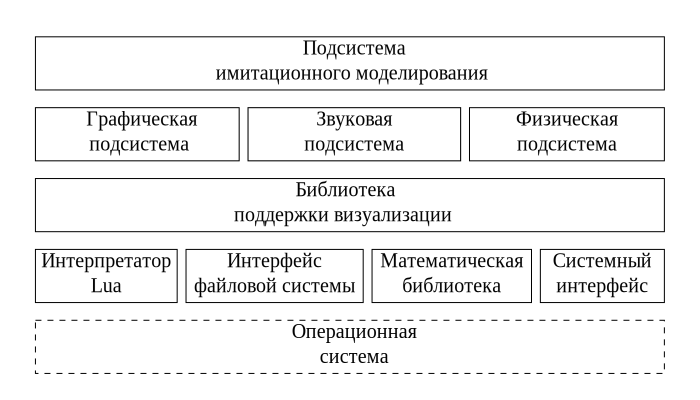
\includegraphics[width=150mm]{system_outline}
	\end{center}
	\caption{Уровни абстракции приложения}
	\label{ship_dfd}
\end{figure}

Следует отметить требования к аппаратному обеспечению. К ним относятся:
\begin{itemize}
	\item	Задачи визуализации и выполнения гидромеханических расчетов необходим 
	видео-ускоритель с поддержкой:
		\begin{itemize}
			\item	Архитектуры CUDA
			\item	Графической библиотеки OpenGL версии 3.3.
			\item	Модели шейдеров  vp40, fp40 --- поддержка расширений \linebreak
			$GL\_NV\_fragment\_program4$ и $GL\_NV\_vertex\_program4$.
		\end{itemize}
	\item	Для задач стерео-визуализации необходимо наличие:
		\begin{itemize}
			\item	Поддержки видео-ускорителем технологии OpenGL quad buffered stereo.
			\item	Наличие средств отображения стерео-контента, 
					таких как стерео-проекторы или стерео-мониторы.
		\end{itemize}	
	\item	Эффективное взаимодействие пользователя с ВП, обеспечивают комплекс устройст ввода, включающий как стандартные мышь и клавиатура, так и более развитые средства, такие как мыши с несколькими степенями свободы.
	\item 	Погружение в акустическую картину виртуального мира необходимо установка звуковой системы объемного звучания. 
\end{itemize}

